\ifx\pdfminorversion\undefined\else\pdfminorversion=4\fi
\documentclass[aspectratio=169,t]{beamer}
%\documentclass[aspectratio=169,t,handout]{beamer}

% English version FAU Logo
\usepackage[english]{babel}
% German version FAU Logo
%\usepackage[ngerman]{babel}

\usepackage[utf8]{inputenc}
\usepackage[T1]{fontenc}
\usepackage{amsmath,amssymb}
\usepackage{graphicx}
\usepackage{listings}
\usepackage{url}
\usepackage{enumitem}
\usepackage{hyperref}
\usepackage{fontawesome}
\usepackage{graphicx}
\usepackage{booktabs}
\usepackage{tikz}
\usepackage{tikz-cd}
\usepackage{pgfplots,pgfplotstable}
\usepackage{filecontents}
\pgfplotsset{compat=1.10}
\newcommand{\plots}{0.611201}
\newcommand{\plotm}{2.19882}
\pgfplotsset{height=4cm,width=8cm,compat=1.16}
\pgfmathdeclarefunction{gauss}{2}{%
  \pgfmathparse{1/(#2*sqrt(2*pi))*exp(-((x-#1)^2)/(2*#2^2))}%
}

\tikzset{
    vertex/.style = {
        circle,
        fill            = black,
        outer sep = 2pt,
        inner sep = 1pt,
    }
}
\usetikzlibrary{matrix,mindmap}
\usetikzlibrary{arrows,decorations.pathmorphing,backgrounds,fit,positioning,shapes.symbols,chains,intersections,snakes}
\tikzset{level 1/.append style={sibling angle=50,level distance = 165mm}}
\tikzset{level 2/.append style={sibling angle=20,level distance = 45mm}}
\tikzset{every node/.append style={scale=1}}
\newcommand{\tikzmark}[1]{\tikz[remember picture] \node[coordinate] (#1) {#1};}
% Options:
%  - inst:      Institute
%                 med:      MedFak FAU theme
%                 nat:      NatFak FAU theme
%                 phil:     PhilFak FAU theme
%                 rw:       RWFak FAU theme
%                 rw-jura:  RWFak FB Jura FAU theme
%                 rw-wiso:  RWFak FB WISO FAU theme
%                 tf:       TechFak FAU theme
%  - image:     Cover image on title page
%  - plain:     Plain title page
%  - longtitle: Title page layout for long title
\usetheme[%
  image,%
  longtitle,%
  tf
]{fau}

% Enable semi-transparent animation preview
\setbeamercovered{transparent}


\lstset{%
  language=Python,
  tabsize=2,
  basicstyle=\tt,
  keywordstyle=\color{blue},
  commentstyle=\color{green!50!black},
  stringstyle=\color{red},
  numbers=left,
  numbersep=0.5em,
  xleftmargin=1em,
  numberstyle=\tt
}


% Title, authors, and date
\title[KDD]{Chapter II: Data}
\subtitle{Knowledge Discovery in Databases}
\author[L.~Melodia]{Luciano Melodia M.A.}
% English version
\institute[Department]{Evolutionary Data Management, Friedrich-Alexander University Erlangen-Nürnberg}
% German version
%\institute[Lehrstuhl]{Lehrstuhl, Friedrich-Alexander-Universit\"at Erlangen-N\"urnberg}
\date{Summer semester 2021}
% Set additional logo (overwrites FAU seal)
%\logo{\includegraphics[width=.15\textwidth]{themefau/art/xxx/xxx.pdf}}
\begin{filecontents}{data.dat}
  2 0.0629921259843
  3 0.0236220472441
  4 0.0314960629921
  5 0.125984251969
  6 0.0629921259843
  7 0.102362204724
  8 0.110236220472
  9 0.0551181102362
  10 0.0629921259843
  11 0.0314960629921
  12 0.0236220472441
  13 0.0314960629921
  14 0.0629921259843
  15 0.0551181102362
  16 0.0393700787402
  17 0.0472440944882
  18 0.00787401574803
  19 0.0393700787402
  24 0.00787401574803
  27 0.00787401574803
  33 0.00787401574803
\end{filecontents}

\begin{document}
\pgfplotstableread{
10.46365192956
90.22330318663
15.4712651178
80.87219994452
90.92824632322
80.69935247007
170.8222081627
140.3601041144
220.9047131581
80.05005282649
90.650706465
170.2352199894
70.76424153088
10.370245979
70.12513239519
20.64730407495
70.2072208982
14.7683650153
14.0063750733
19.324137585
20.40858604381
18.0368674939
80.02681240716
80.26418810694
120.1941169594
90.62080674537
30.24961728242
30.27316960403
170.9038479307
70.40481579419
10.814441695
80.40741573499
60.08031313304
130.1781459953
100.206134367
150.0864695726
90.03013313987
40.46906993699
90.27542593922
110.387166818
50.34088290758
70.35790199406
110.8693581818
100.8557924873
130.969617244
100.6354692297
30.03046442179
60.60358722529
120.2836888554
80.46665782108
130.9221860476
150.1323993544
70.16507829073
50.69317421704
150.4624253296
160.9138444234
60.44259653768
160.4478862876
30.46926929558
100.8862152053
100.4982459647
130.079580222
100.8219448481
120.1887774019
20.27608579327
40.21879129366
80.6626149873
30.05616084556
120.2628717929
30.07385860151
120.1834370192
70.86785100457
220.3039915506
70.6084726129
30.38040559575
40.77264935147
130.9493967532
140.1237678197
60.79956429934
80.7032357113
60.08645967617
90.19491098171
17.1651582777
40.7041931405
30.78091331321
50.20247821499
13.8921717364
60.09560236506
18.5811121283
10.3758110312
80.95955605147
12.4511725524
40.67834498484
11.0234433275
15.364443589
80.23928346825
60.30079928878
90.95330967273
12.5692010856
11.8362767596
}\datatable
\pgfplotstablesort{\sorted}{\datatable}
\pgfplotstablegetrowsof{\datatable}
\edef\numrows{\pgfplotsretval}
  % Title
  \maketitle

  { 
    \setbeamertemplate{footline}{}
    \begin{frame}{Chapter II: Getting to know your data}
    This is our agenda for this lecture:
        \begin{itemize}
            \item \textbf{Data objects and attribute types.}
            \item Basic statistical descriptions of data.
            \item Data visualization.
            \item Measuring data similarity and dissimilarity.
            \item Summary.
        \end{itemize}
    \end{frame}
  }

  { 
    \setbeamertemplate{footline}{}
    \begin{frame}{Types of data sets}
      \begin{columns}
        \begin{column}{0.45\textwidth}
          \textbf{Records:}
          \begin{itemize}[noitemsep]
              \item Relational records.
              \item Data matrix, e.g. numerical matrix, crosstabs.
              \item Document data: text documents, \textbf{term-frequency vectors}. \tikzmark{n1}
              \item \textbf{Transaction data}. \tikzmark{n2}
          \end{itemize}
          \textbf{Graph and network:}
          \begin{itemize}[noitemsep]
              \item World wide web.
              \item Social of information networks.
              \item Molecular structures.
          \end{itemize}
        \end{column}
        \begin{column}{0.45\textwidth}  %%<--- here
        \begin{table}
         \begin{tabular}{|c|c|c|c|c|c|c|}
            \multicolumn{1}{c|}{} & \rotatebox[origin=c]{270}{team} & \rotatebox[origin=c]{270}{couch} & \rotatebox[origin=c]{270}{play} & \rotatebox[origin=c]{270}{ball} & \rotatebox[origin=c]{270}{score} & \rotatebox[origin=c]{270}{game} \\ \hline
            \tikzmark{t1} Document1 & 3 & 0 & 5 & 0 & 2 & 6 \\ \hline
            Document2 & 0 & 7 & 0 & 2 & 1 & 0 \\ \hline
            Document3 & 0 & 1 & 0 & 0 & 1 & 2 \\
            \hline
          \end{tabular}\\[0.5cm]
          \begin{tabular} { | c | l |}
          \hline
          \textbf{TID} & \textbf{Items} \\
          \hline
          \tikzmark{t2} 1 & Bread, Coke, Milk\\
          2 & Beer, Bread\\
          3 & Beer, Coke, Diapers, Milk\\
          4 & Beer, Bread, Diapers, Milk\\
          5 & Coke, Diapers, Milk \\
          \hline
          \end{tabular}
        \end{table}
        \begin{tikzpicture}[remember picture,overlay]
           \path[draw=blue,thick,->]<1-> ([yshift=1mm]n1) -- (t1);
           \path[draw=blue,thick,->]<1-> ([yshift=1mm]n2) -- (t2);
        \end{tikzpicture}
        \end{column}
      \end{columns}
    \end{frame}
  }

  { 
    \setbeamertemplate{footline}{}
    \begin{frame}{Types of data sets}
          \textbf{Ordered data:}
          \begin{itemize}[noitemsep]
              \item Video data: sequences of images.
              \item Temporal data: time series.
              \item Sequential data: transaction sequences.
              \item Genetic sequence data.
          \end{itemize}
          \textbf{Spatial, image and multimedia:}
          \begin{itemize}[noitemsep]
              \item Spatial data: maps.
              \item Image data.
              \item Video data.
          \end{itemize}
    \end{frame}
  }

  { 
    \setbeamertemplate{footline}{}
    \begin{frame}{Important characteristics of structured data}
        \textbf{Dimensionality}:\\
        Curse of dimensionality (sparse high-dimensional data spaces).\\[0.2cm]
        % make the example with the volume of a cube

        \textbf{Sparsity}:\\
        Only presence counts.\\[0.2cm]

        \textbf{Resolution}:\\
        Patterns depend on the scale.\\[0.2cm]

        \textbf{Distribution}:\\
        Centrality and dispersion.
    \end{frame}
  }

  { 
    \setbeamertemplate{footline}{}
    \begin{frame}{Data objects}
      \textbf{Data sets are made up of data objects}.\\
      \textbf{A data object represents an entity}.\\[0.2cm]

      Examples:
      \begin{itemize}
          \item Sales database: customers, store items, sales.
          \item Medical database: patients, treatments.
          \item University database: students, professors, courses.
      \end{itemize}

      They are also called:\\
      Sampels, examples, instances, data points, objects, tuples, \ldots\\[0.2cm]

      \textbf{Data objects are described by attributes}:
      \begin{itemize}
          \item Database rows $\rightarrow$ data objects.
          \item Columns $\rightarrow$ attributes.
      \end{itemize}
    \end{frame}
  }

  { 
    \setbeamertemplate{footline}{}
    \begin{frame}{Attributes}
    \textbf{Attribute}:\\
    Sometimes also in other context: field, dimension, feature, variable, \ldots\\[0.2cm]
    A data field encodes the property of an entity or feature of a data object.\\
    E.g. \texttt{customer\_ID}, \texttt{name}, \texttt{address}.\\[0.5cm]

    \textbf{Types}:
    \begin{itemize}
      \item Nominal.
      \item Binary.
      \item Ordinal.
      \item Numerical:
      \begin{itemize}
        \item Interval scaled.
        \item Ratio scaled.
      \end{itemize}
    \end{itemize}
    \end{frame}
  }

  { 
    \setbeamertemplate{footline}{}
    \begin{frame}{Attribute types}
    \begin{itemize}
        \item \textbf{Nominal}:
        \begin{itemize}
            \item Categories, states, or "names of things".\\
                  E.g. \texttt{hair\_color} $= \{\text{auburn, black, blond, brown, grey, red, white}\}$.\\
                  Other examples: \texttt{marital status}, \texttt{occupation}, \texttt{ID}, \texttt{ZIP code}.
        \end{itemize}
        \item \textbf{Binary}:
            \begin{itemize}
                \item Nominal attribute with only two states ($0$ and $1$).
                \item \textbf{Symmetric binaries}: both outcomes equally important, such as \texttt{gender}.
                \item \textbf{Asymmetric binary}: outcomes not equally important. \\
                      E.g. medical test (positive vs. negative).\\
                      Convention: assign 1 to most important outcome (e.g. HIV positive).
            \end{itemize}
        \item \textbf{Ordinal}:
        \begin{itemize}
            \item Values have a meaningful order (ranking),\\
            but magnitude between successive values is not known.\\
            E.g. \texttt{size} $= \{\text{small, medium, large}\}$, grades, army rankings.
        \end{itemize}
        \end{itemize}
    \end{frame}
  }

  { 
    \setbeamertemplate{footline}{}
    \begin{frame}{Numerical attribute types}
    \begin{itemize}
        \item \textbf{Numerical: Quantity (integer- or real-valued)}.
        \item \textbf{Interval scaled}:
            \begin{itemize}
                \item Measured on a scale of \textbf{equally sized} units.
                \item Values have order.\\
                      E.g. temperature in $C$ or $F$, calender dates.
                \item No true zero-point.
            \end{itemize}
        \item \textbf{Ratio scaled}:
        \begin{itemize}
            \item Inherent \textbf{zero point}.
            \item We can speak of values as being an order of magnitude larger \\
            than the unit of measurement.\\
            E.g. $10 K$ is twice as high as $5 K$.\\
            E.g. temperature in Kelvin, length, counts, monetary quantities.
        \end{itemize}
        \end{itemize}
    \end{frame}
  }

  { 
    \setbeamertemplate{footline}{}
    \begin{frame}{Discrete vs. continuous attributes }
    \begin{itemize}
        \item \textbf{Discrete attribute}:
              \begin{itemize}
                  \item Has finite or countably infinite elements.\\
                        E.g. ZIP code, profession, or the set of words in a collection of documents.
                  \item Sometimes represented as integer variables.
                  \item Note: Binary attributes are a special case of discrete attributes.
              \end{itemize}
        \item \textbf{Continuous attribute}:
            \begin{itemize}
                \item Has real numbers as attribute values.\\
                      E.g. temperature, height, or weight.
                \item Practically, real values can only be measured and represented using a finite number of digits.
                \item Continuous attributes are typically represented as floating-point variables.
            \end{itemize}
        \end{itemize}
    \end{frame}
  }

  { 
    \setbeamertemplate{footline}{}
    \begin{frame}{Chapter II: Getting to know your data}
        \begin{itemize}
            \item Data objects and attribute types.
            \item \textbf{Basic statistical descriptions of data.}
            \item Data visualization.
            \item Measuring data similarity and dissimilarity.
            \item Summary.
        \end{itemize}
    \end{frame}
  }

  { 
    \setbeamertemplate{footline}{}
    \begin{frame}{Basic statistical descriptions of data}
    \textbf{Motivation}:
    \begin{itemize}
      \item To better understand the data: central tendency, variation and spread.
    \end{itemize}

    \textbf{Data dispersion characteristics}:
    \begin{itemize}
        \item Median, max, min, quantiles, outliers, variance etc.
    \end{itemize}

    \textbf{Numerical dimensions correspond to sorted intervals.}\\
    \begin{itemize}
      \item Data dispersion: analyzed with multiple granularities of precision.
      \item Boxplot or quantile analysis on sorted intervals
    \end{itemize}

  \textbf{Dispersion analysis on computed measures.}\\
    \begin{itemize}
        \item Folding measures into numerical dimensions.
        \item Boxplot or quantile analysis on the transformed cube.
    \end{itemize}
    \end{frame}
  }

  { 
    \setbeamertemplate{footline}{}
    \begin{frame}{Measuring the central tendency}
    \begin{itemize}
      \item \textbf{Mean}:
      \begin{itemize}
          \item $N$ denotes the amount of samples within the data set.
          \item The \textbf{sample mean} is given by\\
                \begin{equation*}
                  \bar{x} = \frac{1}{N} \sum_{i=1}^{N} x_i.
                \end{equation*}
          \item While the \textbf{population mean} is defined by
                \begin{equation*}
                  \mu = \sum x \cdot p(x | \theta) \cdots.
                \end{equation*}
      \end{itemize}
    \end{itemize}
    \end{frame}
  }

  { 
    \setbeamertemplate{footline}{}
    \begin{frame}{Measuring the central tendency (2)}
      \begin{columns}
        \begin{column}{0.6\textwidth}
          \textbf{Median:}
          \begin{itemize}[noitemsep]
            \item The median $\tilde{m}$ minimizes the sum of absolute deviations for any $x$ of a sample $X$:
            \begin{align}
              \sum_{i=1}^{n} |\tilde{x}-x_i| \leq \sum_{i=1}^{n} |x-x_i|.
            \end{align}
          \end{itemize}
        \end{column}
        \begin{column}{0.3\textwidth}  %%<--- here
        \begin{table}
        \begin{tabular}{|c|c|}
          Age & Frequency \\ \hline
          $1-5$ & $200$ \\
          $6-15$ & $450$ \\
          $16-20$ & $300$ \\
          $21-50$ & $1500$ \\
          $51-80$ & $700$ \\
          $81-110$ & $44$
        \end{tabular}\\[0.5cm]
        \end{table}
        \end{column}
      \end{columns}
    \end{frame}
  }

  { 
    \setbeamertemplate{footline}{}
    \begin{frame}{Measuring the central tendency (3)}
      \begin{columns}
        \begin{column}{0.6\textwidth}
          \textbf{Median for interval grouped data:}
          \begin{itemize}[noitemsep]
            \item Let $n$ be the total amount of data points, $n_i$ the respective number of the $i$th group and $l_i$ or $u_i$ the lower or upper interval limit. We determine the group to which the median belongs and denote it as $m$th group. It is determined by
            \begin{align}
              \sum_{k=1}^{m-1}n_k < \frac{n}{2}, \; \text{but} \; \sum_{k=1}^{m} n_k \geq \frac{n}{2}.
            \end{align}
            \item If there is no information about the underlying distribution, we just assume that data is equally distributed and use linear interpolation to estimate the median:
            \begin{align}
              \tilde{x} = l_m + \frac{\frac{n}{2}-\sum_{k=1}^{m-1}n_k}{n_m} \cdot (u_m-l_m).
            \end{align}
          \end{itemize}
        \end{column}
        \begin{column}{0.3\textwidth}  %%<--- here
        \begin{table}
        \begin{tabular}{|c|c|}
          Age & Frequency \\ \hline
          $1-5$ & $200$ \\
          $6-15$ & $450$ \\
          $16-20$ & $300$ \\
          $21-50$ & $1500$ \\
          $51-80$ & $700$ \\
          $81-110$ & $44$
        \end{tabular}\\[0.5cm]
        \end{table}
        \end{column}
      \end{columns}
    \end{frame}
  }

  { 
    \setbeamertemplate{footline}{}
    \begin{frame}{Measuring the central tendency (3)}
      \begin{columns}
        \begin{column}{0.6\textwidth}
          \textbf{Mode:}
          \begin{itemize}[noitemsep]
            \item Value that occurs most frequently within the data set.
            \item Can be unimodal, bimodal, trimodal etc.
            \item Empirical formula:
            \begin{align}
              \overline{x} - \text{mode} \approx 3(\overline{x}- \tilde{x}).
            \end{align}
          \end{itemize}
        \end{column}
        \begin{column}{0.3\textwidth}  %%<--- here
        \begin{table}
        \begin{tabular}{|c|c|}
          Age & Frequency \\ \hline
          $1-5$ & $200$ \\
          $6-15$ & $450$ \\
          $16-20$ & $300$ \\
          $21-50$ & $1500$ \\
          $51-80$ & $700$ \\
          $81-110$ & $44$
        \end{tabular}\\[0.5cm]
        \end{table}
        \end{column}
      \end{columns}
    \end{frame}
  }

  { 
    \setbeamertemplate{footline}{}
    \begin{frame}{Example of mode, median and mean}
      \centering
      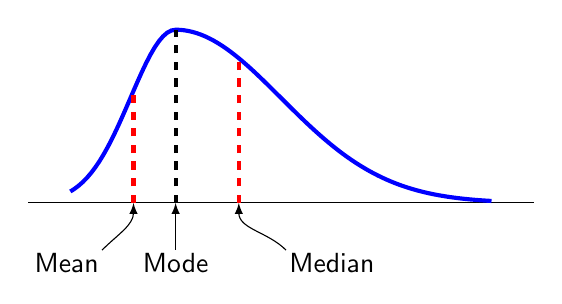
\begin{tikzpicture}[font=\sffamily,
      declare function={Gauss(\x,\y,\z,\u)=1/(\z*sqrt(2*pi))*exp(-((\x-\y+\u*(\x-\y)*sign(\x-\y))^2)/(2*\z^2));},
      every pin edge/.style={latex-,line width=1.5pt},
      every pin/.style={fill=yellow!50,rectangle,rounded corners=3pt,font=\small}]
      \begin{axis}[
          every axis plot post/.append style={
          mark=none,samples=101},
          clip=false,
          axis y line=none,
          axis x line*=bottom,
          ymin=0,
          xtick=\empty,]
          \addplot[line width=1.5pt,blue,domain=-1:3] {Gauss(x,0,0.6,-0.4)};
          \draw[line width=1.5pt,dashed, black] (0,0) -- (0,{Gauss(0,0,0.6,-0.4)});
          \draw[line width=1.5pt,dashed, red] (0.6,0) -- (0.6,{Gauss(0.6,0,0.6,-0.4)});
          \draw[line width=1.5pt,dashed, red] (-0.4,0) -- (-0.4,{Gauss(-0.4,0,0.6,-0.4)});
          \path (-0.4,0) coordinate (ML) (0.6,0) coordinate (MR) (0,0) coordinate (MM);
      \end{axis}
      \draw[latex-] (ML) to[out=-90,in=45] ++ (-0.4,-0.6) node[below left,inner
      sep=1pt]{Mean};
      \draw[latex-] (MR) to[out=-90,in=135] ++ (0.6,-0.6) node[below right,inner
      sep=1pt]{Median};
      \draw[latex-] (MM) --++ (0,-0.6) node[below,inner
      sep=1pt]{Mode};
      \end{tikzpicture}
      \begin{align}
        f(x \vert \mu, \sigma) = \frac{1}{\sqrt{2\pi\sigma^2}} \exp\left( - \frac{(x-\mu)^2}{2\sigma^2}\right).
      \end{align}
    \end{frame}
  }

  { 
    \setbeamertemplate{footline}{}
    \begin{frame}{Example of mode, median and mean}
    \textbf{Quartiles, outliers and boxplots:}
    \begin{itemize}
      \item \textbf{Quartiles:} {\color{blue}$\mathbf{Q}_1$} ($25^{\text{th}}$ percentile), {\color{blue}$\mathbf{Q}_3$} ($75^{\text{th}}$ percentile).
      \item \textbf{Inter quartile range:} {\color{blue}IQR} $=Q_3-Q_1$.
      \item Five number summary: min, $Q_1$, median, $Q_3$, max.
      \item \textbf{Boxplot}: ends of the box are the quartiles; \\ median is marked; add whiskers and plot outliers individually.
      \item \textbf{Outlier}: usually assigned to values higher/lower than $1.5 \cdot \text{IQR}$.
    \end{itemize}
    \textbf{Variance $\sigma^2$ and standard deviation $\sigma$}:
    \begin{itemize}
      \item Empirical sample variance: $\overline{\sigma^2} = \frac{1}{n} \sum_{i=1}^{n}(x_i-\overline{x})^2$
      \item Empirical population variance: $\sigma^2 = \frac{1}{N} \sum_{i=1}^{n} (x_i - \mu)^2$.
      \item Standard deviation is the square root $\sigma = \sqrt{\sigma^2}$.
    \end{itemize}
    \end{frame}
  }

  { 
    \setbeamertemplate{footline}{}
    \begin{frame}{Boxplot analysis}
    \begin{center}
        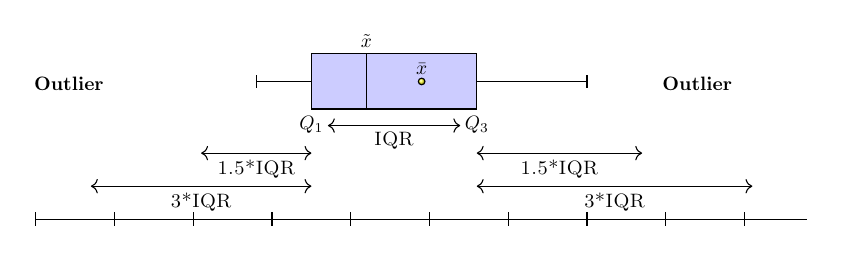
\begin{tikzpicture}[scale=0.7, transform shape]
            \filldraw[fill=blue!20] (2,0) rectangle (5,1);% draw the box
            \draw (3,0) -- (3,1) node[above]{$\tilde{x}$};% draw the median
            \draw (5,0.5) -- (7,0.5);% draw right whisker
            \draw (2,0.5) -- (1,0.5);% draw left whisker
            \draw (7,0.39) -- (7,0.61);% draw vertical tab
            \draw (1,0.39) -- (1,0.61);% draw vertical tab
            \node[below] at (2,0) {$Q_1$};% label the hinge
            \node[below] at (5,0) {$Q_3$};% label the hinge
            \filldraw[ball color=yellow!80,shading=ball] (4,0.5) circle
                (0.06cm) node[above]{$\bar{x}$};% the mean
            \draw[<->] (2.3, -0.3) -- (4.7, -0.3)
                node[pos=0.5,below]{$\textsc{IQR}$}; % mark the IQR fences
            \draw[<->] (2, -0.8) -- (0,-0.8)
                node[pos=0.5,below]{$\textsc{1.5*IQR}$}; % left inner fence
            \draw[<->] (2,-1.4) -- (-2, -1.4)
                node[pos=0.5,below]{$\textsc{3*IQR}$};% left outer fence
            \draw[<->] (5, -0.8) -- (8,-0.8)
                node[midway,below]{$\textsc{1.5*IQR}$}; % right inner fence
            \draw[<->] (5,-1.4) -- (10, -1.4)
                node[pos=0.5,below]{$\textsc{3*IQR}$};% right outer fence
            %
            \node[below] at (9,0.7) {$\textbf{Outlier}$}; % mild outlier on the right
            \node[below] at (-2.4,0.7) {$\textbf{Outlier}$}; % extreme outlier on the left
            % Axis
            \draw (-3,-2) -- (11,-2);
            % Note that the snaked line is drawn to 11.1 to force
            % TikZ to draw the final tick.
            \draw[snake=ticks,segment length=1cm] (-3,-2) -- (11.1,-2);
        \end{tikzpicture}
        \end{center}
          \textbf{Five number summary of a distribution:}\\
          Minimum, $Q_1$, median, $Q_3$, maximum.
          \\[0.2cm]
          \textbf{Boxplot}:
          \begin{itemize}
            \item Data is represented with a box.
            \item The ends of the box are at the first and third quartiles, i.e. the height of the box is IQR. \\
            The median is marked by a line within the box.
            \item Whiskers: two lines outside the box extended to minimum and maximum.
            \item Outliers: points beyond a specified outlier threshold, plotted individually.
          \end{itemize}
    \end{frame}
  }

  { 
    \setbeamertemplate{footline}{}
    \begin{frame}{Properties of normal distribution curves}
    \begin{itemize}
        \item \textbf{The normal distribution:}
        \begin{itemize}
          \item From $\mu - \sigma$ to $\mu + \sigma$: contains about $68\%$ of the measurements.
          \begin{itemize}
              \item $\mu$: mean,
              \item $\sigma$: standard deviation.
          \end{itemize}
          \item From $\mu - 2 \sigma$ to $\mu + 2\sigma$: contains about $95\%$ of the surface under the curve.
          \item $\mu-3\sigma$ to $\mu + 3\sigma$: contains about $99.7\%$ of the surface under the curve.
        \end{itemize}
    \end{itemize}
    \vspace{0.2cm}
    \centering
    \begin{tikzpicture}
    \begin{axis}[
      no markers, domain=-3:3, samples=100,
      axis lines*=left, xlabel=$x$, ylabel=$y$,
      height=3.5cm, width = 5cm,
      xtick={-3,-2,-1,0,1,2,3}, ytick=\empty,
      enlargelimits=false, clip=false, axis on top,
      grid = major
      ]
      \addplot [fill=blue!20, draw=none, domain=-1:1] {gauss(0,1)} \closedcycle;
      \addplot [very thick,blue!50!black] {gauss(0,1)};
      \node[below] at (0,0.15) {$\approx 66 \%$}; 
    \end{axis}
    \end{tikzpicture}
    \hspace{0.2cm}
    \begin{tikzpicture}
    \begin{axis}[
      no markers, domain=-3:3, samples=100,
      axis lines*=left, xlabel=$x$, ylabel=$y$,
      height=3.5cm, width = 5cm,
      xtick={-3,-2,-1,0,1,2,3}, ytick=\empty,
      enlargelimits=false, clip=false, axis on top,
      grid = major
      ]
      \addplot [fill=blue!20, draw=none, domain=-2:2] {gauss(0,1)} \closedcycle;
      \addplot [very thick,blue!50!black] {gauss(0,1)};
      \node[below] at (0,0.15) {$\approx 95 \%$}; 
    \end{axis}
    \end{tikzpicture}
    \hspace{0.2cm}
    \begin{tikzpicture}
    \begin{axis}[
      no markers, domain=-3:3, samples=100,
      axis lines*=left, xlabel=$x$, ylabel=$y$,
      height=3.5cm, width = 5cm,
      xtick={-3,-2,-1,0,1,2,3}, ytick=\empty,
      enlargelimits=false, clip=false, axis on top,
      grid = major
      ]
      \addplot [fill=blue!20, draw=none, domain=-2.97:2.97] {gauss(0,1)} \closedcycle;
      \addplot [very thick,blue!50!black] {gauss(0,1)};
      \node[below] at (0,0.15) {$\approx 99.7 \%$}; 
    \end{axis}
    \end{tikzpicture}
    \hspace{0.2cm}
    \end{frame}
  }

{
  \setbeamertemplate{footline}{}
  \begin{frame}{Visualization of basic statistical descriptions}
  \begin{itemize}
    \item \textbf{Boxplot}: Visualization of five number summary.
    \item \textbf{Histogram}: $x$-axis are values, $y$-axis represent frequencies.
    \item \textbf{Quantile plot}: Each value $x_i$ is paired with some $q_i$ indicating that approximately $q_i \cdot 100 \%$ of data are $\leq x_i$.
    \item \textbf{Quantile-quantile (q-q) plot}: Graphs the quantiles of one univariate distribution against the corresponding quantiles of another.
    \item \textbf{Scatter plot}: Each pair of values is a pair of coordinates and plotted as points in the plane.
  \end{itemize}
  \end{frame}
}

{
  \setbeamertemplate{footline}{}
  \begin{frame}{Histogram analysis}
  \begin{itemize}
    \item \textbf{Histogram}: Visualization of tabulated frequencies, shown as bars.
    \item It shows what proportion of cases fall into each of several categories.
    \item Differs from a $\textbf{bar chart}$ in that it is the \emph{area} of the bar that denotes the value, not the height as in bar charts, a crucial distinction when the categories are not of uniform width.
    \item The categories are usually specified as non-overlapping intervals of some variable. The categories (bars) must be adjacent.
  \end{itemize}\vspace{0.2cm}
  \centering
  \begin{tikzpicture}
    \begin{axis}[
    yticklabel style={/pgf/number format/fixed},
    scaled y ticks = false,
    minor y tick num={1},
    xtick pos=left,
    legend cell align = left,
    legend style={draw=none},
    xlabel = {group size},
    ylabel = {ratio}
    ]
    \addplot[blue,ybar,fill, fill opacity=0.3, bar width = 0.8,] table {data.dat};
    \addplot[red, line width = 1,domain=1:40,samples=100] {1/(x*sqrt(2*pi)*\plots)*exp(-(ln(x)-\plotm)^2/(2*\plots^2))};
    \legend{empirical,lognormal fit}
    \end{axis}
  \end{tikzpicture}
  \end{frame}
}

{
  \setbeamertemplate{footline}{}
  \begin{frame}{Histograms often tell more than boxplots}
  The two histograms shown below may have the same boxplot representation, thus the same values for min, $Q_1$, median, $Q_3$ and for the max. But they have rather different underlying distributions.\\[1cm]
  \centering
  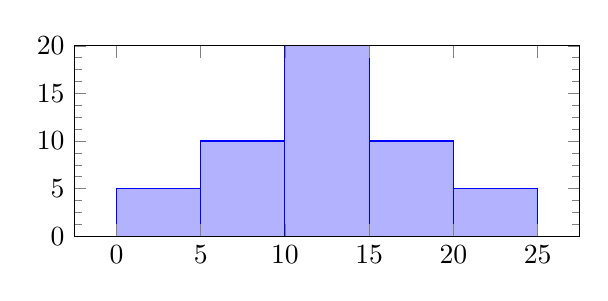
\begin{tikzpicture}
  \begin{axis}[
      ymin=0, ymax=20,
      minor y tick num = 3,
      area style,
      ]
  \addplot+[ybar interval,mark=no] plot coordinates {(0, 5) (5, 10) (10, 20) (15,10) (20,5) (25,5)};
  \end{axis}
  \end{tikzpicture}
  \hspace{0.5cm}
  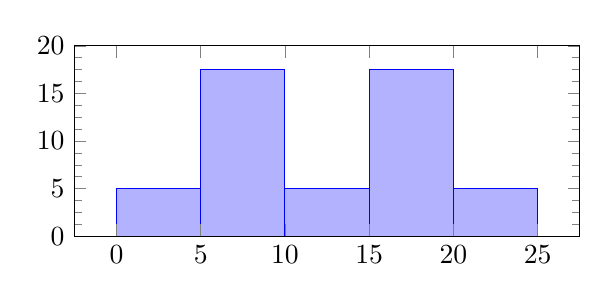
\begin{tikzpicture}
  \begin{axis}[
      ymin=0, ymax=20,
      minor y tick num = 3,
      area style,
      ]
  \addplot+[ybar interval,mark=no] plot coordinates {(0, 5) (5, 17.5) (10, 5) (15,17.5) (20,5) (25,5)};
  \end{axis}
  \end{tikzpicture}
  \end{frame}
}

  { 
    \setbeamertemplate{footline}{}
    \begin{frame}{Quantile plot}
    \textbf{Displays all of the data.}\\
    A quantile plot allows the user to assess both the overall behaviour and unusual occurrences.\\[0.5cm]
    \textbf{Plots quantile information.}\\
    For some data point $x_i$, sorted in increasing order, $q_i$ indicates that approximately $q_i \cdot 100 \%$ of the data are below or equal to the value of $x_i$.\\[0.2cm]
    \centering
    \begin{tikzpicture}[
        declare function={norm(\x)=\x*\x/200;},
    ]
    \begin{axis}[
      ylabel={Unit price in \$},
      xlabel={q-value},
    ]
    \addplot table [x index=0, y index=0, x expr = \coordindex/150, y expr=norm(\coordindex)] {\sorted};
    \end{axis}
    \end{tikzpicture}
    \end{frame}
  }

  { 
    \setbeamertemplate{footline}{}
    \begin{frame}{Quantile-quantile (q-q) plot}
    \begin{itemize}
      \item Graphs the quantiles of one univariate distribution against the corresponding quantiles of another.
      \item View: Is there is a shift in going from one distribution to another?\\
      Example shows unit price of items sold at Branch $1$ vs. branch $2$ for each quantile.  Unit prices of items sold at branch $1$ tend to be lower than those at branch $2$.
    \end{itemize}\vspace{0.5cm}
    \centering
    \begin{tikzpicture}[
        declare function={norm(\x)=2*\x;},
    ]
    \begin{axis}[
      ylabel={Branch 2 (unit price in \$)},
      xlabel={Branch 1 (unit price in \$)},
    ]
    \addplot [only marks, mark=*] table [x index=0, y index=0, y expr=norm(\coordindex)] {\sorted};
    \draw[black, thick] (0,0) -- (200,200);
    \end{axis}
    \end{tikzpicture}
    \end{frame}
  }

  { 
    \setbeamertemplate{footline}{}
    \begin{frame}{References I}

    \end{frame}
  }

  { 
    \setbeamertemplate{footline}{}
    \begin{frame}{References I}
        \begin{itemize}
          \item W. Cleveland: Visualizing Data, Hobart Press, 1993.
          \item T. Dasu and T. Johnson: Exploratory Data Mining and Data Cleaning, John Wiley, 2003.
          \item U. Fayyad, G. Grinstein, and A. Wierse: Information Visualization in Data Mining and Knowledge Discovery, Morgan Kaufmann, 2001.
          \item L. Kaufman and P. J. Rousseeuw: Finding Groups in Data: an Introduction to Cluster Analysis, John Wiley \& Sons, 1990.
          \item H. V. Jagadish et al.: Special Issue on Data Reduction Techniques, Bulletin of the Tech. Committee on Data Eng., 20(4), 1997.
          \item D. Keim: Information visualization and visual data mining, IEEE Trans. on Visualization and Computer Graphics, 8(1), 2002.
          \item F. Naumann: Data Profiling Revisited, ACM SIGMOD Record, 32(4), 2013, 40-49.
          \item D. Pyle: Data Preparation for Data Mining, Morgan Kaufmann, 1999.
        \end{itemize}
    \end{frame}
  }

  { 
    \setbeamertemplate{footline}{}
    \begin{frame}{References II}
        \begin{itemize}
          \item S.  Santini and R. Jain: Similarity measures, IEEE Trans. on Pattern Analysis and Machine Intelligence, 21(9), 1999.
          \item E. R. Tufte: The Visual Display of Quantitative Information, 2nd ed., Graphics Press, 2001.
          \item C. Yu et al.: Visual data mining of multimedia data for social and behavioral studies, Information Visualization, 8(1), 2009.
        \end{itemize}
    \end{frame}
  }

  { % Questions?
    \setbeamertemplate{footline}{}
    \begin{frame}[c]
      \begin{center}
        Thank you for your attention.\\
        {\bf Any questions about the second chapter?}\\[0.5cm]
        Ask them now, or again, drop me a line: \\ 
        \faSendO \ \texttt{luciano.melodia@fau.de}.
      \end{center}
    \end{frame}
  }
\end{document}

